\begin{frame}[c, parent={cmap:software-testing}, hasprev=false, hasnext=true]
\frametitle{JUnit}
\label{cmap:junit}

\insertcmap{Courses-SoftwareTesting-JUnit}
\end{frame}


\begin{frame}[c, parent={cmap:software-testing}, hasprev=true, hasnext=false]
\frametitle{JUnit}
\centering
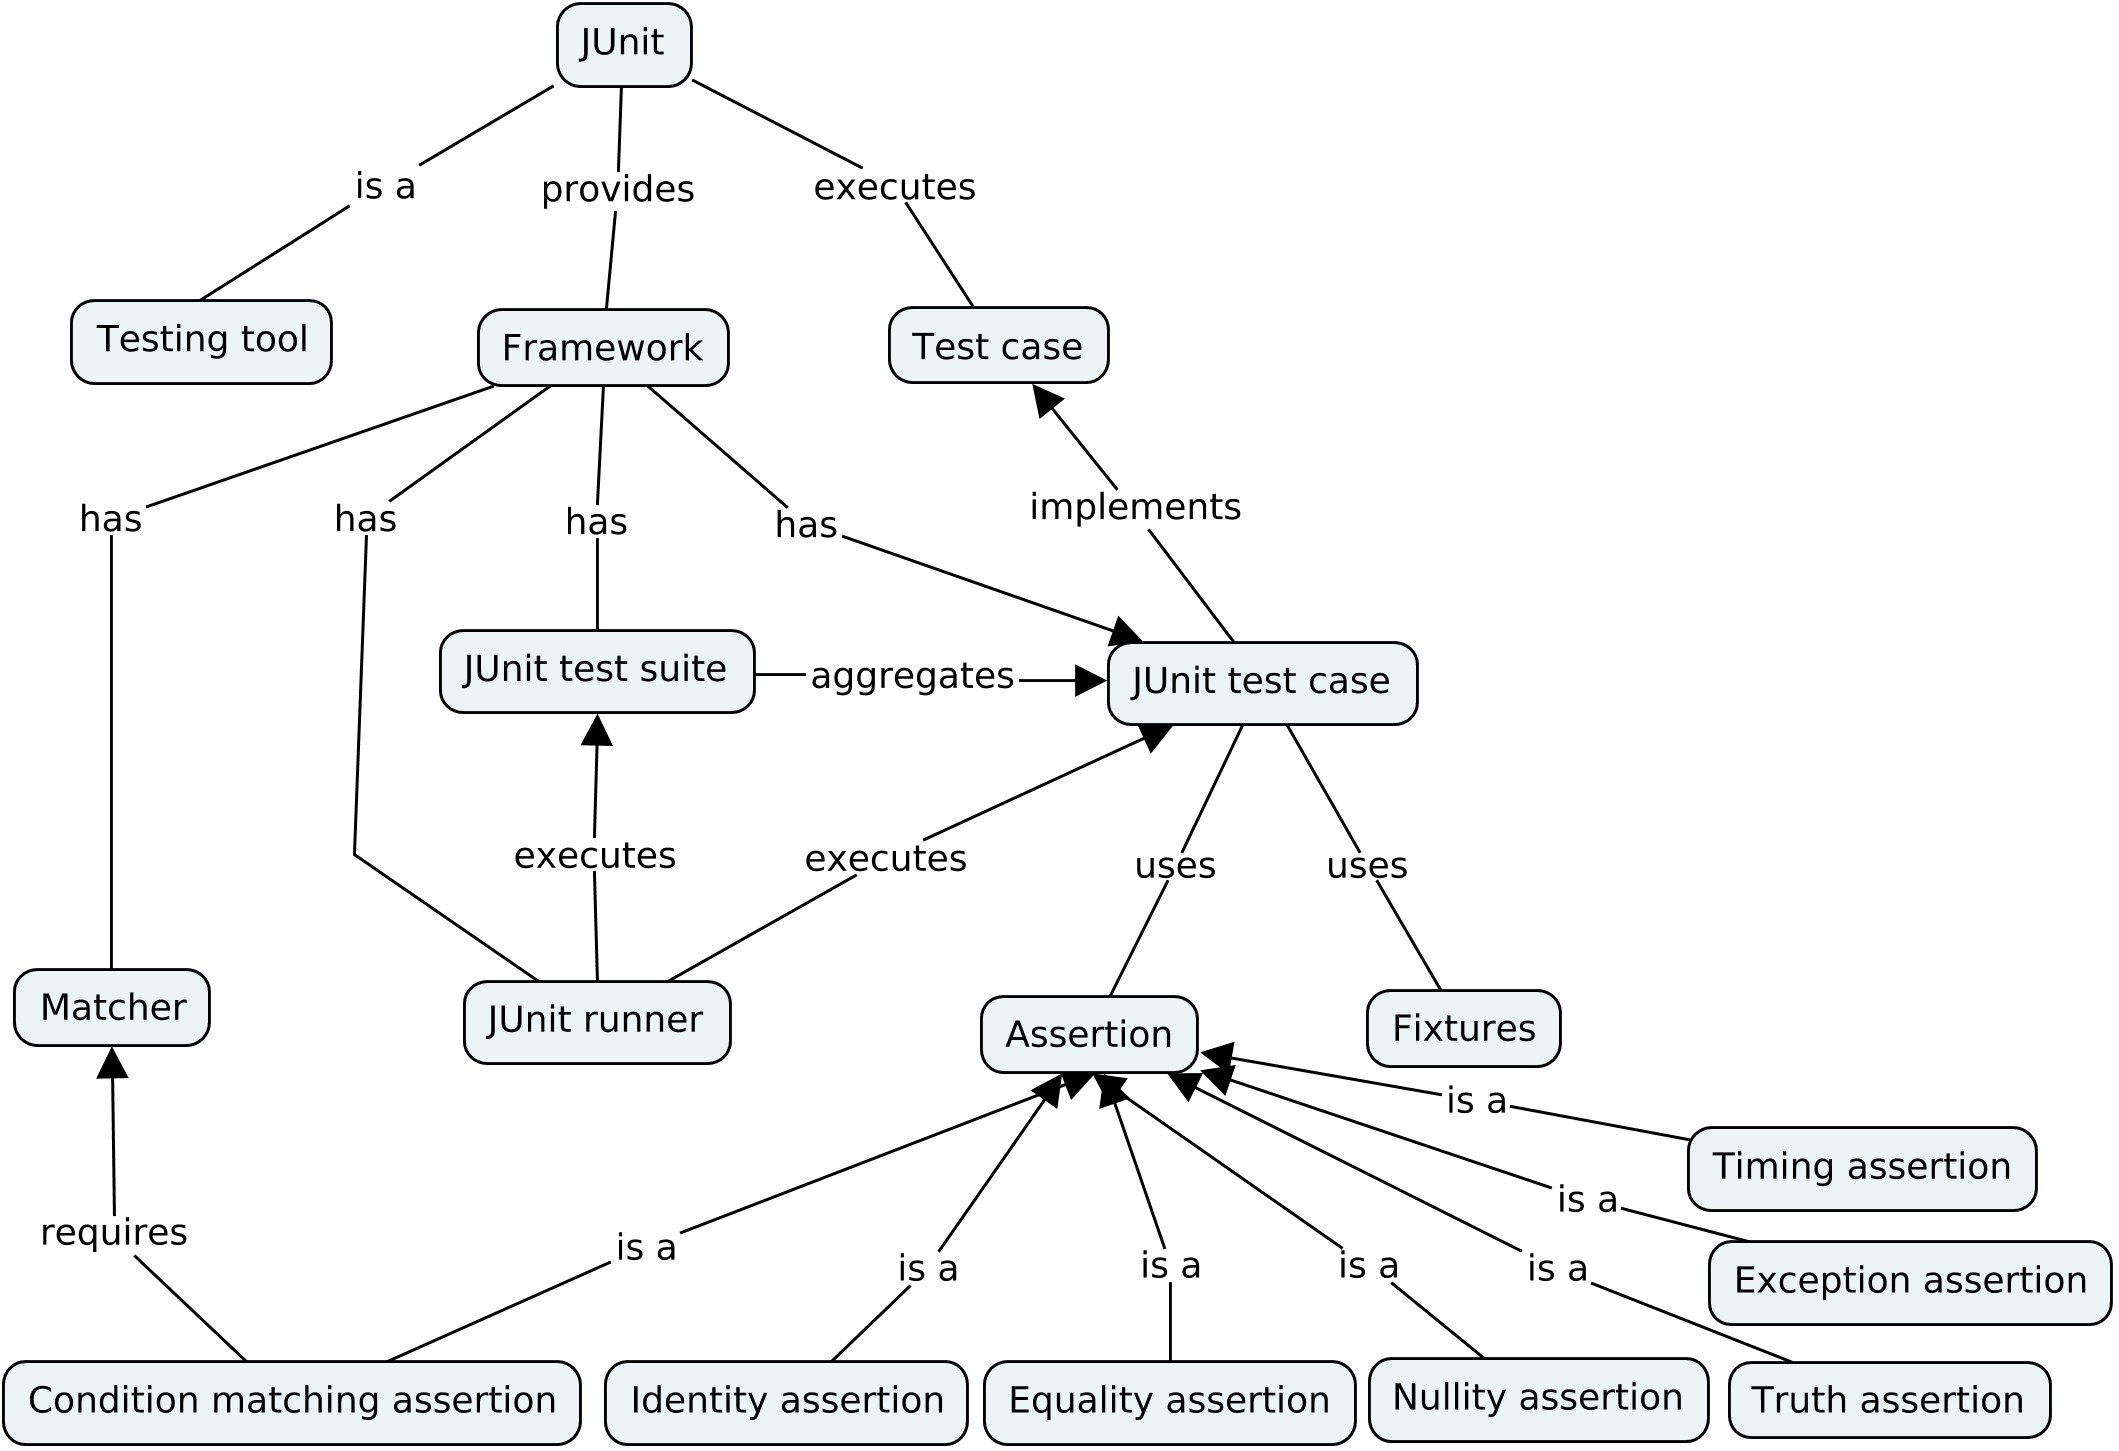
\includegraphics[width=\textwidth]{JUnit.jpg}
\end{frame}


\begin{frame}[parent={cmap:junit}, hasprev=false, hasnext=true]
\frametitle{JUnit}
\label{concept:junit}

\begin{block:concept}{What is it?}
JUnit is an open-source framework to provide support for documenting and
automating the execution of test sets for Java programs.
\end{block:concept}


\begin{block:fact}{General information}
\begin{itemize}
	\item Developed by Kent Beck and Erich Gamma (in 1994).

	\item Hosted at \url{https://www.junit.org/} and
	\url{https://github.com/junit-team/junit4}.
\end{itemize}
\end{block:fact}


\begin{block:fact}{Features}
\begin{itemize}
	\item Test cases implemented using annotations.

	\item Useful assertions collection.

	\item Fixtures enhances the design of test sets.
\end{itemize}
\end{block:fact}

\hfill
\refie{example:identifier-testcases-junit}{\beamerbutton{Example: Identifier}}
\end{frame}



